\documentclass{article}
\usepackage[b5paper, margin=1in]{geometry}

% colored links
\usepackage{hyperref}
\hypersetup{
    colorlinks=true,
    linkcolor=blue,
    filecolor=magenta,      
    urlcolor=magenta,
    }

%Creating algorithms
\usepackage{algorithm}
\usepackage[noend]{algpseudocode}
% \renewcommand\algorithmicthen{}
\renewcommand\algorithmicdo{}

\usepackage{fancyhdr}
\usepackage{enumitem}
\usepackage{extramarks}
\usepackage{amsmath}
\usepackage{amsthm}
\usepackage{amsfonts}
\usepackage{tikz}
\usetikzlibrary{arrows.meta, shapes, positioning}
% \usepackage[plain]{algorithm}
\usepackage{algpseudocode}

\usetikzlibrary{automata,positioning}
\usetikzlibrary{shapes.geometric}
\usetikzlibrary{positioning,calc}


\newcommand{\enterProblemHeader}[1]{
    \nobreak\extramarks{}{Problem \arabic{#1} continued on next page\ldots}\nobreak{}
    \nobreak\extramarks{Problem \arabic{#1} (continued)}{Problem \arabic{#1} continued on next page\ldots}\nobreak{}
}

\newcommand{\exitProblemHeader}[1]{
    \nobreak\extramarks{Problem \arabic{#1} (continued)}{Problem \arabic{#1} continued on next page\ldots}\nobreak{}
    \stepcounter{#1}
    \nobreak\extramarks{Problem \arabic{#1}}{}\nobreak{}
}

\setcounter{secnumdepth}{0}
\newcounter{partCounter}
\newcounter{homeworkProblemCounter}
\setcounter{homeworkProblemCounter}{1}
\nobreak\extramarks{Fall 2022 %\arabic{homeworkProblemCounter}
}{}\nobreak{}

%
% Homework Problem Environment
%
% This environment takes an optional argument. When given, it will adjust the
% problem counter. This is useful for when the problems given for your
% assignment aren't sequential. See the last 3 problems of this template for an
% example.
%
\newenvironment{homeworkProblem}[1][-1]{
    \ifnum#1>0
        \setcounter{homeworkProblemCounter}{#1}
    \fi
    \section{Problem \arabic{homeworkProblemCounter}}
    \setcounter{partCounter}{1}
    \enterProblemHeader{homeworkProblemCounter}
}{
    \exitProblemHeader{homeworkProblemCounter}
}

\begin{document}


\section*{Problem 2 Solution}

\begin{enumerate}
    \item The following list of steps demonstrate the push-relabel algorithm

    \begin{center}
        \begin{tabular}{r | l}
            R & DTW from $h = 0$ to $h = 1$ \\
            P & 15 from DTW to BOS \\
            R & BOS from $h = 0$ to $h = 1$ \\
            P & 15 from BOS to ATL \\
            R & JFK from $h = 0$ to $h = 1$ \\
            P & 15 from JFK to ATL \\
            R & MIA from $h = 0$ to $h = 1$ \\
            P & 15 from MIA to ATL \\
            R & PHX from $h = 0$ to $h = 1$ \\
            P & 16 from PHX to JFK \\
            R & JFK from $h = 1$ to $h = 2$ \\
            P & 15 from JFK to MIA \\
            P & 5 from JFK to PHX \\
            R & PHX from $h = 1$ to $h = 2$ \\
            P & 16 from PHX to MIA \\
            R & MIA from $h = 1$ to $h = 2$ \\
            P & 26 from MIA to ATL \\
            P & 5 from MIA to BOS \\
            P & 5 from BOS to ATL \\
            Rx6 & PHX from $h = 2$ to $h = 8$ \\
            P & 2 from PHX to LAX
        \end{tabular}
    \end{center}
\end{enumerate}

\begin{itemize}
    \item[(a)] The network below represents the (hypothetical) connections between a number of international airports, where the capacity of an edge represents the maximum number of flights that can be scheduled between two airports on a given day.

    \vspace{2mm} Imagine an urgent situation, like a massive concert or a sports event suddenly announced in Atlanta, has just caused a surge of travelers needing to fly from Los Angeles (LAX) to Atlanta (ATL) ASAP. The big question is: how many flights can actually make this journey in a single day without overstretching the system?
    
    \vspace{2mm} Run the Push-Relabel Algorithm to answer this question. Along with your final numerical answer, include the following:
    \begin{enumerate}[label=\roman*.]
        \item A sketch of the final residual graph with the accompanying capacities (indicate edges in $E^{f} \setminus E$ with dashed lines), as well as the final heights of each node.
        \item The number of times the \verb+Push+ subroutine has been called, as well as the number of times the \verb+Relabel+ subroutine was called.
    \end{enumerate}
    \textbf{In the case of ties, choose the node with the smallest lexicographical order.}
    \begin{center}
        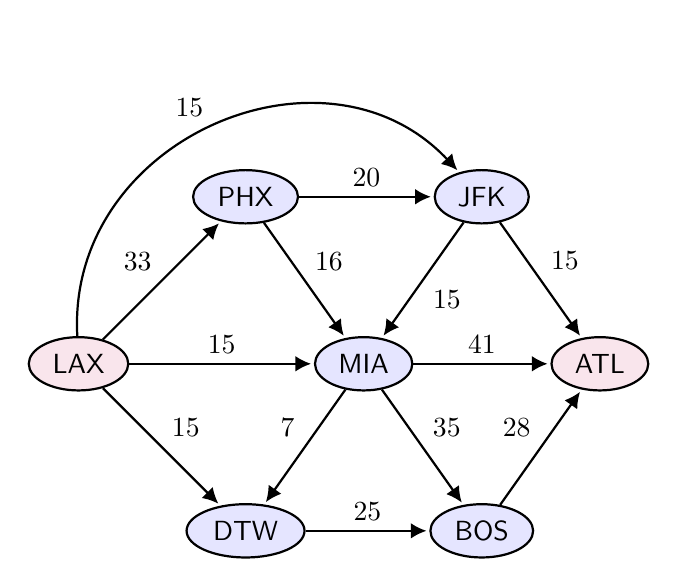
\begin{tikzpicture}[
            % scale=0.8,
            % transform shape,
            shorten >=1pt,
            node distance=3cm,
            auto,
            thick, % makes the lines a bit thicker
            font=\sffamily, % changes the font to sans-serif
            every state/.style={
                shape=ellipse,
                fill=blue!10,
                minimum size=0.5cm,
                thick
            },
            every edge/.style={
                draw,
                -{Latex[length=2mm, width=2mm]} % makes arrow tips a bit nicer
            }
        ]
        \node[state, fill = purple!10] (a) [] {LAX};
        \node[state] (b) [above right of=a] (b) {PHX};
        \node[state] (c) [below right of=a] (c) {DTW};
        \node[state] (d) [right of=b] (d) {JFK};
        \node[state] (e) at ($(a -| b)!0.5!(a -| d)$) {MIA};
        \node[state] (f) [right of=c] (f) {BOS};
        \node[state, fill = purple!10] (g) [right of=e] (g) {ATL};
        \path[->]
            (a) edge node {$33$} (b)
            (a) edge node {$15$} (c)
            (a) edge [bend left=1cm, out=70, in=110, distance=2.5cm] node {$15$} (d)
            (a) edge node {$15$} (e)
            (b) edge node {$20$} (d)
            (b) edge node {$16$} (e)
            (c) edge node {$25$} (f)
            (d) edge node {$15$} (e)
            (d) edge node {$15$} (g)
            (e) edge node[above left] {$7$} (c)
            (e) edge node {$35$} (f)
            (e) edge node {$41$} (g)
            (f) edge node {$28$} (g);
    \end{tikzpicture}
    \end{center}
    \item[(b)] A basic implementation of the algorithm in the exposition gives us a runtime of $\mathcal{O}(mn^{2})$. Give an implementation of this algorithm that runs in $\mathcal{O}(n^{3})$ time, and prove the runtime of your algorithm.

    \vspace{2mm} \textit{Hints: first prove the running time bound assuming that, in each iteration, you can identify the highest vertex with positive excess in O(1) time. The hard part is to maintain the vertices with positive excess in a data structure such that, summed over all of the iterations of the algorithm, only $\mathcal{O}(n^{3})$ total time is used to identify these vertices.}
    \item[(c)] \textit{(Optional)} It can be shown (with a little more work) that a tight bound for this algorithm is $\Theta(n^{2}\sqrt{m})$\footnote{Asymptotically, a $\sqrt{m}$ term is better than a $n$ term.}. Although this bound is nothing special in the worst-case (for example, Dinic's algorithm runs in time $\mathcal{O}(nm^{2})$, the PR algorithm is often the one used.\footnote{This dichotomy with theoretical bounds and practical application is oftentimes the case with flow-based networks; for example, in \href{https://www.csd.uwo.ca/~yboykov/Papers/pami04.pdf}{computer vision}.} What are some reasons why this algorithm may perform better in practice?
\end{itemize}

\end{document}